\documentclass[preprint, 3p,
authoryear]{elsarticle} %review=doublespace preprint=single 5p=2 column
%%% Begin My package additions %%%%%%%%%%%%%%%%%%%

\usepackage[hyphens]{url}

  \journal{Geographical Analysis} % Sets Journal name

\usepackage{lineno} % add
  \linenumbers % turns line numbering on

\usepackage{graphicx}
%%%%%%%%%%%%%%%% end my additions to header

\usepackage[T1]{fontenc}
\usepackage{lmodern}
\usepackage{amssymb,amsmath}
\usepackage{ifxetex,ifluatex}
\usepackage{fixltx2e} % provides \textsubscript
% use upquote if available, for straight quotes in verbatim environments
\IfFileExists{upquote.sty}{\usepackage{upquote}}{}
\ifnum 0\ifxetex 1\fi\ifluatex 1\fi=0 % if pdftex
  \usepackage[utf8]{inputenc}
\else % if luatex or xelatex
  \usepackage{fontspec}
  \ifxetex
    \usepackage{xltxtra,xunicode}
  \fi
  \defaultfontfeatures{Mapping=tex-text,Scale=MatchLowercase}
  \newcommand{\euro}{€}
\fi
% use microtype if available
\IfFileExists{microtype.sty}{\usepackage{microtype}}{}
\usepackage[]{natbib}
\bibliographystyle{plainnat}

\ifxetex
  \usepackage[setpagesize=false, % page size defined by xetex
              unicode=false, % unicode breaks when used with xetex
              xetex]{hyperref}
\else
  \usepackage[unicode=true]{hyperref}
\fi
\hypersetup{breaklinks=true,
            bookmarks=true,
            pdfauthor={},
            pdftitle={Reproducibility of research during COVID-19: examining the case of population density and the basic reproductive rate from the perspective of spatial analysis},
            colorlinks=false,
            urlcolor=blue,
            linkcolor=magenta,
            pdfborder={0 0 0}}

\setcounter{secnumdepth}{0}
% Pandoc toggle for numbering sections (defaults to be off)
\setcounter{secnumdepth}{0}


% tightlist command for lists without linebreak
\providecommand{\tightlist}{%
  \setlength{\itemsep}{0pt}\setlength{\parskip}{0pt}}



\usepackage{booktabs}
\usepackage{longtable}
\usepackage{array}
\usepackage{multirow}
\usepackage{wrapfig}
\usepackage{float}
\usepackage{colortbl}
\usepackage{pdflscape}
\usepackage{tabu}
\usepackage{threeparttable}
\usepackage{threeparttablex}
\usepackage[normalem]{ulem}
\usepackage{makecell}
\usepackage{xcolor}



\begin{document}


\begin{frontmatter}

  \title{Reproducibility of research during COVID-19: examining the case
of population density and the basic reproductive rate from the
perspective of spatial analysis}
    \author[McMaster University]{Antonio Paez%
  \corref{cor1}%
  }
   \ead{paezha@mcmaster.ca} 
      \affiliation[McMaster University]{School of Earth, Environment and
Society, 1280 Main St West, Hamilton, Ontario L8S 4K1 Canada}
    \cortext[cor1]{Corresponding author}
  
  \begin{abstract}
  The emergence of the novel SARS-CoV-2 coronavirus and the global
  COVID-19 pandemic in 2019 led to explosive growth in scientific
  research. Alas, much of the research in the literature lacks
  conditions to be reproducible, and recent publications on the
  association between population density and the basic reproductive
  number of SARS-CoV-2 are no exception. Relatively few papers share
  code and data sufficiently, which hinders not only verification but
  additional experimentation. In this paper, an example of reproducible
  research shows the potential of spatial analysis for epidemiology
  research during COVID-19. Transparency and openness means that
  independent researchers can, with only modest efforts, verify findings
  and use different approaches as appropriate. Given the high stakes of
  the situation, it is essential that scientific findings, on which good
  policy depends, are as robust as possible; as the empirical example
  shows, reproducibility is one of the keys to ensure this.

  This paper is now published in Geographical Analysis
  (\url{https://doi.org/10.1111/gean.12307})
  \end{abstract}
    \begin{keyword}
    keyword1 \sep 
    keyword2
  \end{keyword}
  
 \end{frontmatter}

\newpage

\hypertarget{introduction}{%
\section{Introduction}\label{introduction}}

The emergence of the novel SARS-CoV-2 coronavirus in 2019, and the
global pandemic that followed in its wake, led to an explosive growth of
research around the globe. According to Fraser et al.
\citeyearpar{Fraser2021evolving}, over 125,000 COVID-19-related papers
were released in the first ten months from the first confirmed case of
the disease. Of these, more than 30,000 were shared in pre-print
servers, the use of which also exploded in the past year
\citep{Kwon2021swamped, Vlasschaert2020proliferation, Anazco2021publication}.

Given the ruinous human and economic cost of the pandemic, there has
been a natural tension in the scientific community between the need to
publish research results quickly and the imperative to maintain
consistently high quality standards in scientific reporting; indeed, a
call for maintaining the standards in published research termed the
deluge of COVID-19 publications a ``carnage of substandard research''
\citep{Bramstedt2020carnage}. Part of the challenge of maintaining
quality standards in published research is that, despite an abundance of
recommendations and guidelines
\citep[e.g.,][]{Broggini2017reproducible, Ince2012case, Ioannidis2014increasing, Brunsdon2020opening},
in practice reproducibility has remained a lofty and somewhat
aspirational goal
\citep{Konkol2019examination, Konkol2019computational}. As reported in
the literature, only a woefully small proportion of published research
was actually reproducible before the pandemic
\citep{Iqbal2016reproducible, Stodden2018empirical}, and the situation
does not appear to have changed substantially since
\citep{Sumner2020reproducibility, Gustot2020quality}.

The push for open software and data
\citep[e.g.,][]{Bivand2020progress, Arribas2021open}, along with more
strenuous efforts towards open, reproducible research, is simply a
continuation of long-standing scientific practices of independent
verification. Despite the (at times disproportionate) attention that
high profile scandals in science tend to elicit in the media, science as
a collective endeavor is remarkable for being a self-correcting
enterprise, one with built-in mechanisms and incentives to weed out
erroneous ideas. Over the long term, facts tend to prevail in science.
At stake is the shorter-term impacts that research may have in other
spheres of economic and social life. The case of economists Reinhart and
Rogoff comes to mind: by the time the inaccuracies and errors in their
research were uncovered \citep[see][]{Herndon2014high}, their claims
about debt and economic growth had already been seized by policy-makers
on both sides of the Atlantic to justify austerity policies in the
aftermath of the Great Recession of 2007-2009\footnote{Nobel Prize in
  Economics Paul Krugman noted that ``Reinhart--Rogoff may have had more
  immediate influence on public debate than any previous paper in the
  history of economics''
  \url{https://www.nybooks.com/articles/2013/06/06/how-case-austerity-has-crumbled/?pagination=false}}.
As later research has demonstrated, those policies cast a long shadow,
and their sequels continued to be felt for years \citep{Basu2017ten}.

In the context of COVID-19, a topic that has grabbed the imagination of
numerous thinkers has been the prospect of life in cities after the
pandemic \citep[e.g.,][]{Florida2020how}; as a result, the implications
of the pandemic for urban planning, design, and management are the topic
of ongoing research \citep[e.g.,][]{Sharifi2020covid}. The fact that the
worst of the pandemic was initially felt in dense population centers
such as Wuhan, Milan, Madrid, and New York, unleashed a torrent of
research into the associations between density and the spread of the
pandemic. The answers to some important questions hang on the results of
these research efforts. For example, are lower density regions safer
from the pandemic? Are de-densification policies warranted, even if just
in the short term? In the longer term, will the risks of life in high
density regions presage a flight from cities? And, what are the
implications of the pandemic for future urban planning and practice?
Over the past year, numerous papers have sought to throw light on the
underlying issue of density and the pandemic; nonetheless the results,
as will be detailed next, remain mixed. Further, to complicate matters,
precious few of these studies appear to be sufficiently open to support
independent verification.

The objective of this paper is to illustrate the importance of
reproducibility in research in the context of the flood of COVID-19
papers. For this, I focus on a recent study by Sy et al.
\citeyearpar{Sy2021population} that examined the correlation between the
basic reproductive number of COVID-19, \(R_0\), and population density.
The basic reproductive number is a summary measure of contact rates,
probability of transmission of a pathogen, and duration of
infectiousness. In rough terms, it measures how many new infections each
infections begets. The paper of Sy et al. \citeyearpar{Sy2021population}
was selected for being, in the literature examined, almost alone in
supporting reproducible research. Accordingly, I wish to be clear that
my objective in singling their work for discussion is not to malign
their efforts, but rather to demonstrate how open and reproducible
research efforts can greatly help to accelerate discovery. More
concretely, open data and open code mean that an independent researcher
can, with only modest efforts, not only verify the findings reported,
but also examine the same data from a perspective which may not have
been available to the original researchers due to differences in
disciplinary perspectives, methodological traditions, and/or training,
among other possible factors. The example, which shows consequential
changes in the conclusions reached by different analyses, should serve
as a call to researchers to redouble their efforts to increase
transparency and reproducibility in their research. In this spirit, the
present paper also aims to show how data can be packaged in
well-documented, shareable units, and code can be embedded into
self-contained documents suitable for review and independent
verification. The source for this paper is an
\href{http://rmarkdown.rstudio.com}{R Markdown} document which, along
with the data package, are available in a public repository\footnote{\url{https://github.com/paezha/Reproductive-Rate-and-Density-US-Reanalyzed}}.

\hypertarget{background-the-intuitive-relationship-between-density-and-spread-of-contagious-diseases}{%
\section{Background: the intuitive relationship between density and
spread of contagious
diseases}\label{background-the-intuitive-relationship-between-density-and-spread-of-contagious-diseases}}

The concern with population density and the spread of the virus during
the COVID-19 pandemic was fueled, at least in part, by dramatic scenes
seen in real-time around the world from large urban centers such as
Wuhan, Milan, Madrid, and New York. In theory, there are good reasons to
believe that higher density could have a positive association with the
transmission of a contagious virus. It has long been known that the
potential for inter-personal contact is greater in regions with higher
density \citep[see for example the research on urban fields and
time-geography,
including][]{Farber2011running, Moore1970urban, Moore1970some}.
Mathematically, models of exposure and contagion indicate that higher
densities can catalyze the transmission of contagious diseases
\citep{Rocklov2020high, Li2018effect}. The idea is intuitive and likely
at the root of messages, by some figures in positions of authority, that
regions with sparse population densities faced lower risks from the
pandemic\footnote{Governor Kristi Noem of South Dakota, for example,
  claimed that sparse population density allowed her state to face the
  pandemic down without the need for strict policy interventions
  \url{https://www.inforum.com/lifestyle/health/5025620-South-Dakota-is-not-New-York-City-Noem-defends-lack-of-statewide-COVID-19-restrictions}}.

As Rocklöv and Sjödin \citep{Rocklov2020high} note, however,
mathematical models of contagion are valid at small-to-medium spaces
(and presumably, smaller time intervals too, such as time spent in
restaurants, concert halls, cruises), and the results do not necessarily
transfer to larger spatial units and longer time periods. There are
solid reasons for this: while in a restaurant, one can hardly avoid
being in proximity to other customers. On the other hand, a person can
choose to (or be forced to as a matter of policy) not go to a restaurant
in the first place. Nonetheless, the idea that high density correlates
with high transmission is so seemingly sensible that it is often taken
for granted even at the scale of large spaces
\citep[e.g.,][]{Cruz2020exploring, Micallef2020first}. In such
conditions, however, there exists the possibility of behavioral
adaptations, which are difficult to capture in the mechanistic framework
of differential equations \citep[or can be missing in agent-based
models, e.g.,][]{Gomez2021infekta}; these adaptations, in fact, can be a
key aspect of disease transmission.

A plausible behavioral adaptation during a pandemic, especially one
broadcast as widely and intensely as COVID-19, is risk compensation.
Risk compensation is a process whereby people adjust their behavior in
response to their \emph{perception} of risk
\citep{Noland1995perceived, Richens2000condoms, Phillips2011risk}. In
the case of COVID-19, Chauhan et al. \citep{Chauhan2021covid} have found
that perception of risks in the US varies between rural, suburban, and
urban residents, with rural residents in general expressing less concern
about the virus. It is possible that people who listened to the message
of leaders saying that they were safe from the virus because of low
density may not have taken adequate precautions. Conversely, people in
dense places who could more directly observe the impact of the pandemic
may have become overly cautious. Both Paez et al.
\citeyearpar{Paez2020spatio} and Hamidi et al.
\citeyearpar{Hamidi2020density} posit this mechanism (i.e., greater
compliance with social distancing in denser regions) to explain the
results of their analyses. The evidence available does indeed show that
there were important changes in behavior with respect to mobility during
the pandemic
\citep{Jamal2020Changes, Harris2021Changes, Molloy2020Tracing};
furthermore, shelter in place orders may have had greater buy-in from
the public in higher density regions
\citep{Feyman2020effectiveness, Hamidi2021compact}, and the associated
behavior may have persisted beyond the duration of official
social-distancing policies \citep{Praharaj2020Using}. In addition, there
is evidence that changes in mobility correlated with the trajectory of
the pandemic \citep{Paez2020using, Noland2021mobility}. Given the
potential for behavioral adaptation, the question of density becomes
more nuanced: it is not just a matter of proximity, but also of human
behavior, which is better studied using population-level data and
models.

\hypertarget{background-but-what-does-the-literature-say}{%
\section{Background: but what does the literature
say?}\label{background-but-what-does-the-literature-say}}

When it comes to population density and the spread of COVID-19, the
international literature to date remains inconclusive.

On the one hand, there are studies that report positive associations
between population density and various COVID-19-related outcomes. Bhadra
\citeyearpar{Bhadra2021impact}, for example, reported a moderate
positive correlation between the spread of COVID-19 and population
density at the district level in India, however their analysis was
bivariate and did not control for other variables, such as income.
Similarly, Kadi and Khelfaoui \citeyearpar{Kadi2020population} found a
positive and significant correlation between number of cases and
population density in cities in Algeria in a series of simple regression
models (i.e., without other controls). A question in these relatively
simple analyses is whether density is not a proxy for other factors.
Other studies have included controls, such as Pequeno et al.
\citeyearpar{Pequeno2020air}, a team that reported a positive
association between density and cumulative counts of confirmed COVID-19
cases in state capitals in Brazil after controlling for covariates,
including income, transport connectivity, and economic status. In a
similar vein, Fielding-Miller et al. \citeyearpar{Fielding2020social}
reported a positive relationship between the absolute number of COVID-19
deaths and population density (rate) in rural counties in the US. Roy
and Ghosh \citeyearpar{Roy2020factors} used a battery of machine
learning techniques to find discriminatory factors, and a positive and
significant association between COVID-19 infection and death rates in US
states. Wong and Li \citeyearpar{Wong2020spreading} also found a
positive and significant association between population density and
number of confirmed COVID-19 cases in US counties, using both univariate
and multivariate regressions with spatial effects. More recently, Sy et
al. \citeyearpar{Sy2021population} reported that the basic reproductive
number of COVID-19 in US counties tended to increase with population
density, but at a decreasing rate at higher densities.

On the flip side, a number of studies report non-significant or negative
associations between population density and COVID-19 outcomes. This
includes the research of Sun et al. \citeyearpar{Sun2020impacts} who did
not find evidence of significant correlation between population density
and confirmed number of cases per day \emph{in conditions of lockdown}
in China. This finding echoes the results of Paez et al.
\citeyearpar{Paez2020spatio}, who in their study of provinces in Spain
reported non-significant associations between population density and
infection rates in the early days of the first wave of COVID-19, and
negative significant associations in the later part of the first
lockdown. Similarly, \citet{Skorka2020macroecology} found zero or
negative associations between population density and infection
numbers/deaths by country. Fielding-Miller et al.
\citeyearpar{Fielding2020social} contrast their finding about rural
counties with a negative relationship between COVID-19 deaths and
population density in urban counties in the US. For their part, in their
investigation of doubling time, White and Hébert-Dufresne
\citeyearpar{White2020state} identified a negative and significant
correlation between population density and doubling time in US states.
Likewise, \citet{Khavarian2021high} found a small negative (and
significant) association between population density and COVID-19
morbidity in districts in Tehran. Finally, two of the most complete
studies in the US, by \citet{Hamidi2020longitudinal} and
\citet{Hamidi2020density}, used an extensive set of controls to find
negative and significant correlations between density and COVID-19 cases
and fatalities at the level of counties in the US.

As can be seen, these studies are implemented at different scales in
different regions of the world. They also use a range of techniques,
from correlation analysis, to multivariate regression, spatial
regressions, and machine learning techniques. This is natural and to be
expected: individual researchers have only limited time and expertise.
This is why reproducibility is important. To pick an example (which will
be further elaborated in later sections of this paper), the study of Sy
et al. \citeyearpar{Sy2021population}, hereafter referred to as SWN,
would immediately grab the attention of a researcher with expertise in
spatial analysis.

\hypertarget{reproducibility-of-research}{%
\section{Reproducibility of
research}\label{reproducibility-of-research}}

SWN investigated the basic reproductive number of COVID-19 in US
counties, and its association with population density, median household
income, and prevalence of private mobility. For their multivariate
analysis, SWN used mixed linear models. This is an appropriate modelling
choice: \(R_0\) is an interval-ratio variable that is suitably modeled
using linear regression; further, as SWN note there is a likelihood that
the process in not independent ``among counties within each state,
potentially due to variable resource allocation and differing health
systems across states'' (p.~3). A mixed linear model accounts for this
by introducing random components; in the case of SWN, these are random
intercepts at the state level. SWN estimated various models with
different combinations of variables, including median household income
and prevalence of travel by private transportation. These controls help
to account for potential variations in behavior: people in more affluent
counties may have greater opportunities to work from home, and use of
private transportation reduces contact with strangers. Moreover, they
also conducted various sensitivity analyses. After these efforts, SWN
concluded that there is a positive association between the basic
reproductive number and population density at the level of counties in
the US.

One salient aspect of the analysis in SWN is that the basic reproductive
number can only be calculated reliably with a minimum number of cases,
and a large number of counties did not meet such threshold. As
researchers do, SWN made modelling decisions, in this case basing their
analysis only on counties with valid observations. A modeler with
expertise in spatial analysis would likely ask some of the following
questions on reading SWN's paper: how were missing counties treated?
What are the implications of the spatial sampling framework used in the
analysis? Is it possible to spatially interpolate the missing
observations? Was there spatial residual autocorrelation in the models,
or was the use of mixed models sufficient to capture spatial
dependencies? These questions are relevant and their implications
important. Fortunately, SWN are an example of a reasonably open,
reproducible research product: their paper is accompanied by (most of)
the data and (most of) the code used in the analysis. This means that an
independent researcher can, with only a moderate investment of time and
effort, reproduce the results in the paper, as well as ask additional
questions.

Alas, reproducibility is not necessarily the norm in the relevant
literature.

There are various reasons why a project can fail to be reproducible. In
some cases, there might be legitimate reasons to withhold the data,
perhaps due to confidentiality and privacy reasons
\citep[e.g.,][]{Lee2020human}. But in many other cases the data are
publicly available, which in fact has commonly been the case with
population-level COVID-19 information. Typically the provenance of the
data is documented, but in numerous studies the data themselves are not
shared
\citep{Amadu2021assessing, Bhadra2021impact, Cruz2020exploring, Feng2020spread, Fielding2020social, Hamidi2020longitudinal, Hamidi2020density, Inbaraj2021seroprevalence, Souris2020covid}.
As any researcher can attest, collecting, organizing, and preparing data
for a project can take a substantial amount of time. Pointing to the
sources of data, even when these sources are public, is a small step
towards reproducibility-but only a very small one. Faced with the
prospect of having to recreate a data set from raw sources is probably
sufficient to dissuade all but the most dedicated (or stubborn)
researcher from independent verification. This is true even if part of
the data are shared \citep[e.g.,][]{Wong2020spreading}. In other cases,
data are shared, but the processes followed in the preparation of the
data are not fully documented
\citep{Ahmad2020association, Skorka2020macroecology}. These processes
matter, as shown by the errors in the spreadsheets of Reinhart and
Rogoff \citep[see][ for the discovery of these errors]{Herndon2014high},
as well as by the data of biologist Jonathan Pruitt that led to an
``avalanche'' of paper retractions \citep[see][]{Viglione2020avalanche}.
Another situation is when papers share well-documented data, but fail to
provide the code used in the analysis
\citep{Noury2021how, Pequeno2020air, Wang2021transmission}. Making code
available only ``on demand'' \citep[e.g.,][]{Brandtner2021creatures} is
an unnecessary barrier when most journals offer the facility to share
supplemental materials online. Then there are those papers that more
closely comply with reproducibility standards, and share well-documented
processes and data, as well as the code used in any analyses reported
\citep{Paez2020spatio, Feyman2020effectiveness, Stephens2021impact, White2020state, Sy2021population}.
Even in this case, the pressure to publish ``new findings'' instead of
replication studies can act as a deterrent, perhaps particularly for
younger researchers\footnote{The present paper was desk rejected by
  three journals that had previously published research on population
  density and the spread of COVID-19; in one case, the paper was too
  opinionated for the journal, in the other two cases, the paper was not
  a ``good fit'' despite dealing with a nearly identical issue as papers
  previously published in said journals.}.

In the following sections, the analysis of SWN is reproduced, some
relevant questions from the perspective of an independent researcher
with expertise in spatial analysis are asked, and the data are
reanalyzed.

\hypertarget{reproducing-swn}{%
\section{Reproducing SWN}\label{reproducing-swn}}

SWN examined the association between the basic reproductive number of
COVID-19 and population density. The basic reproductive number \(R_0\)
is a summary measure of contact rates, probability of transmission of a
pathogen, and duration of infectiousness. In rough terms, \(R_0\)
measures how many new infections each infections begets. Infectious
disease outbreaks generally tend to die out when \(R_0<1\), and to grow
when \(R_0>1\). Reliable calculation of \(R_0\) requires a minimum
number of cases to be able to assume that there is community
transmission of the pathogen. Accordingly, SWN based their analysis only
on counties that had at least 25 cases or more at the end of the
exponential growth phase (see Fig. \ref{fig:R0-map}). Their final sample
included 1,151 counties in the US, including in Alaska, Hawaii, Puerto
Rico, and island territories. SWN used COVID-19 data collected by the
New York Times and made available (with versioning) in a GitHub
repository\footnote{https://github.com/nytimes/covid-19-data}. For each
county, SWN assumed that the exponential growth period began one week
prior to the second daily increase in cases, and assumed that the period
of exponential growth lasted approximately 18 days.

\begin{figure}
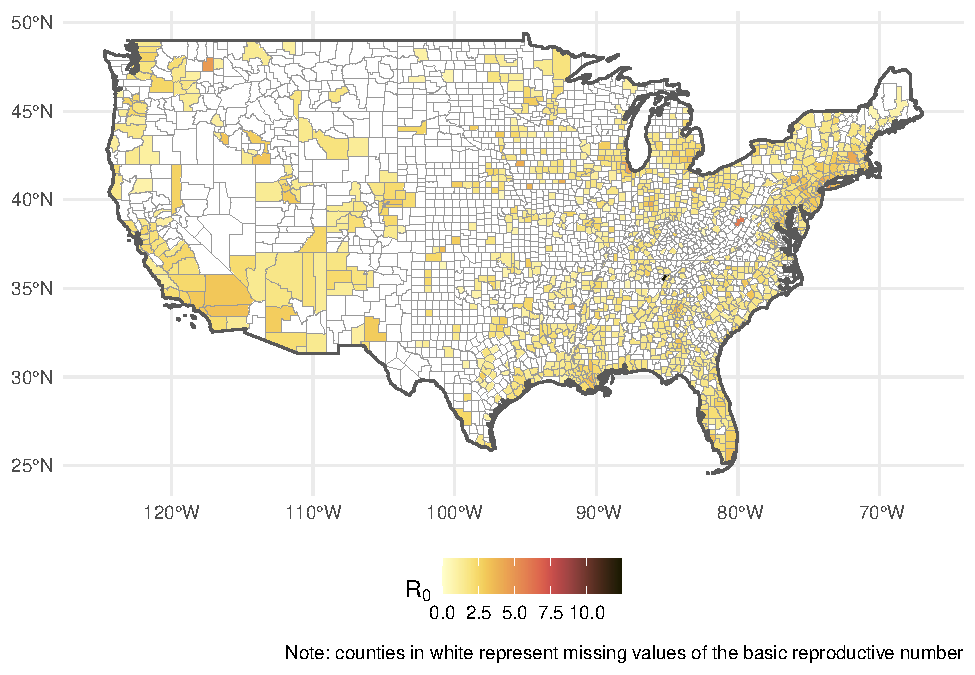
\includegraphics[width=1\linewidth]{R0-Density-Reanalysis_files/figure-latex/R0-map-1} \caption{\label{fig:R0-map}Basic reproductive rate in US counties (Alaska, Hawaii, Puerto Rico, and territories not shown).}\label{fig:R0-map}
\end{figure}

Table \ref{tab:swn-results} reproduces the first three models of SWN
(the fourth model did not have any significant variables; see Table 1 in
SWN). It is possible to verify that the results match, with only the
minor (and irrelevant) exception of the magnitude of the coefficient for
travel by private transportation, which is due to a difference in the
input (here the variable is changed to one percent units, instead of the
ten percent units used by SWN). The mixed linear model gives random
intercepts (i.e., the intercept is a random variable), and the standard
deviation is reported in the fifth row of Table \ref{tab:swn-results}.
It is useful to map the random intercepts: as seen in Figure
\ref{fig:random-terms-map}, other things being equal, counties in Texas
tend to have somewhat lower values of \(R_0\) (i.e., a negative random
intercept), whereas counties in South Dakota tend to have higher values
of \(R_0\). The key of the analysis, after extensive sensitivity
analysis, is a robust finding that population density has a positive
association with the basic reproductive number. But does it?

\begin{table}

\caption{\label{tab:tabulate-swn-results}\label{tab:swn-results}Reproducing SWN: Models 1-3}
\centering
\resizebox{\linewidth}{!}{
\begin{tabular}[t]{lllllrl}
\toprule
\multicolumn{1}{c}{ } & \multicolumn{2}{c}{Model 1} & \multicolumn{2}{c}{Model 2} & \multicolumn{2}{c}{Model 3} \\
\cmidrule(l{3pt}r{3pt}){2-3} \cmidrule(l{3pt}r{3pt}){4-5} \cmidrule(l{3pt}r{3pt}){6-7}
Variable & beta & 95\% CI & beta & 95\% CI & beta & 95\% CI\\
\midrule
Intercept & 2.274 & {}[2.167, 2.381] & 3.347 & {}[2.676, 4.018] & 3.386 & {}[2.614, 4.157]\\
Log of population density & 0.162 & {}[0.133, 0.191] & 0.145 & {}[0.115, 0.176] & 0.147 & {}[0.113, 0.18]\\
Percent of private transportation &  &  & -0.013 & {}[-0.02, -0.005] & -0.013 & {}[-0.021, -0.005]\\
Median household income (\$10,000) &  &  &  &  & -0.003 & {}[-0.033, 0.026]\\
Standard deviation (Intercept) & 0.166 & {}[0.108, 0.254] & 0.136 & {}[0.081, 0.229] & 0.137 & {}[0.081, 0.232]\\
\addlinespace
Within-group standard error & 0.665 & {}[0.638, 0.693] & 0.665 & {}[0.638, 0.693] & 0.665 & {}[0.638, 0.694]\\
\bottomrule
\end{tabular}}
\end{table}

\begin{figure}
\includegraphics[width=1\linewidth]{R0-Density-Reanalysis_files/figure-latex/random-terms-map-1} \caption{\label{fig:random-terms-map}Random intercepts of Model 3 (Alaska, Hawaii, Puerto Rico, and territories not shown).}\label{fig:random-terms-map}
\end{figure}

\hypertarget{expanding-on-swn}{%
\section{Expanding on SWN}\label{expanding-on-swn}}

The preceding section shows that thanks to the availability of code and
data, it is possible to verify the results reported by SWN. As noted
earlier, though, an independent researcher might have wondered about the
implications of the spatial sampling procedure used by SWN. The decision
to use a sample of counties with reliable basic reproductive numbers,
although apparently sensible, results in a non-random spatial sampling
scheme. Turning our attention back to Figure \ref{fig:R0-map}, we form
the impression that many counties without reliable values of \(R_0\) are
in more rural, less dense parts of the United States. This impression is
reinforced when we overlay the boundaries of urban areas with population
greater than 50,000 on the counties with valid values of \(R_0\) (see
Figure \ref{fig:urban-areas-map}). The fact that \(R_0\) could not be
accurately computed in many counties without large urban areas does not
mean that there was no transmission of the virus: it simply means that
we do not know with sufficient precision to what extent that was the
case. The low number of cases may be related to low population and/or
low population density. This is intriguing, to say the least: by
excluding cases based on the ability to calculate \(R_0\) we are
potentially \emph{selecting} the sample in a non-random way.

\begin{figure}
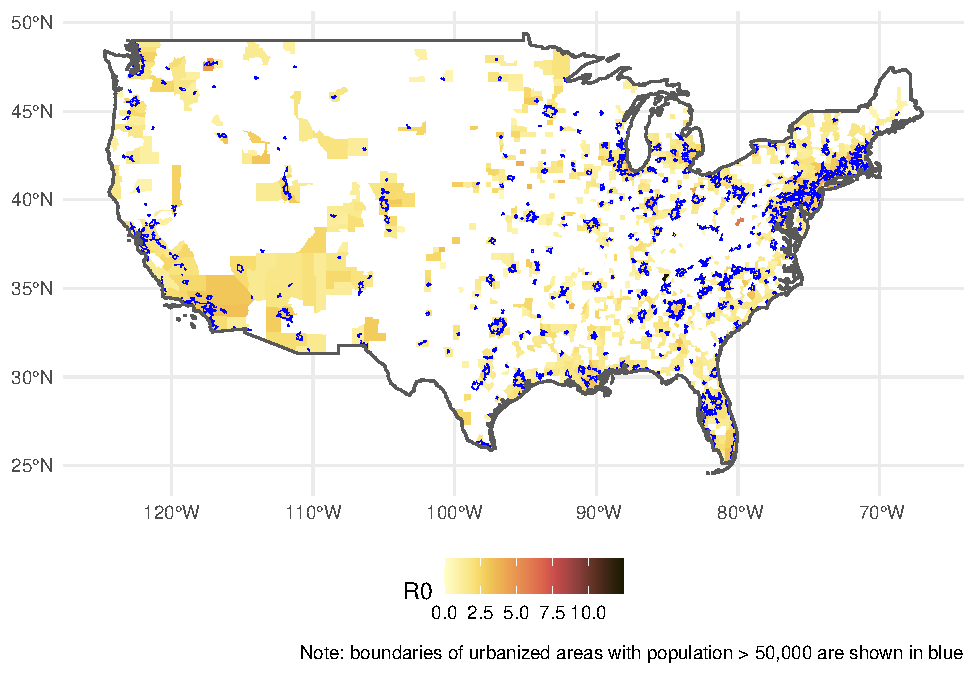
\includegraphics[width=1\linewidth]{R0-Density-Reanalysis_files/figure-latex/urban-areas-map-1} \caption{\label{fig:urban-areas-map}Urban areas with population > 50,000 (Alaska, Hawaii, Puerto Rico, and territories not shown).}\label{fig:urban-areas-map}
\end{figure}

A problematic issue with non-random sample selection is that parameter
estimates can become unreliable, and numerous techniques have been
developed to address this. A model useful for sample selection problems
is Heckman's selection model \citep[see][]{Maddala1983limited}. The
selection model is in fact a system of two equations, as follows: \[
\begin{array}{c}
y_i^{S*} = \beta^{S\prime}x_i^S+\epsilon_i^S\\
y_i^{O*} = \beta^{O\prime}x_i^O+\epsilon_i^O
\end{array}
\] \noindent where \(y_i^{S*}\) is a latent variable for the sample
selection process, and \(y_i^{O*}\) is the latent outcome. Vectors
\(x_i^S\) and \(x_i^O\) are explanatory variables (with the possibility
that \(x_i^S = x_i^S\)). Both equations include random terms (i.e.,
\(\epsilon_i^S\) and \(\epsilon_i^O\)). The first equation is designed
to model the \emph{probability} of sampling, and the second equation the
outcome of interest (say \(R_0\)). The random terms are jointly
distributed and correlated with parameter \(\rho\).

What the analyst observes is the following: \[
y_i^S =
\begin{cases}
0 & \text{if } y_i^{S*} < 0\\
1 & \text{otherwise}
\end{cases}
\] \noindent and: \[
y_i^O =
\begin{cases}
0 & \text{if } y_i^{S} = 0\\
y_i^{O*} & \text{otherwise}
\end{cases}
\]

In other words, the outcome of interest is observed \emph{only} for
certain cases (\(y_i^S=1\), i.e., for sampled observations). The
probability of sampling depends on \(x_i^S\). For the cases observed,
the outcome \(y_i^O\) depends on \(x_i^O\).

A sample selection model is estimated using the same selection of
variables as SWN Model 3. This is Sample Selection Model 1 in Table
\ref{tab:selection-results}. The first thing to notice about this model
is that the sample selection process and the outcome are correlated
(\(\rho\ne0\) with 5\% of confidence). The selection equation indicates
that the probability of a county to be in the sample increases with
population density (but at a decreasing rate due to the
log-transformation), when travel by private modes is more prevalent, and
as median household income in the county is higher. This is in line with
the impression made by Figure \ref{fig:urban-areas-map} that counties
with reliable values of \(R_0\) tended to be those with larger urban
centers. Once that the selection probabilities are accounted for in the
model, several things happen with the outcomes model. First, the
coefficient for population density is still positive, but the magnitude
changes: in effect, it appears that the effect of density is more
pronounced than what SWN Model 3 indicated. The coefficient for percent
of private transportation changes signs. And the coefficient for median
household income is now significant.

The second model in Table \ref{tab:selection-results} (Selection Model
2) changes the way the variables are entered into the model. The
log-transformation of density in SWN and Selection Model 1 assumes that
the association between density and \(R_0\) is monotonically increasing
(if the sign of the coefficient is positive) or decreasing (if the sign
of the coefficient is negative). There are some indications that the
relationship may actually not be monotonical. For example, Paez et al.
\citeyearpar{Paez2020spatio} found a positive (if non-significant)
relationship between density and incidence of COVID-19 in the provinces
of Spain at the beginning of the pandemic. This changed to a negative
(and significant) relationship during the lockdown. In the case of the
US, Fielding-Miller et al. \citeyearpar{Fielding2020social} found that
the association between COVID-19 deaths and population density was
positive in rural counties, but negative in urban counties. A variable
transformation that allows for non-monotonic changes in the relationship
is the square of the density.

As seen in the table, Selection Model 2 replaces the log-transformation
of population density with a quadratic expansion. The results of this
analysis indicate that with this variable transformation, the selection
and outcome processes are still correlated (\(\rho\ne0\) with 5\% of
confidence). But a few other interesting things emerge. When we examine
the outcomes model, we see that the quadratic expansion has a positive
coefficient for the first order term, but a negative coefficient for the
second order term. This indicates that \(R_0\) initially tends to
increase as density grows, but only up to a point, after which the
negative second term (which grows more rapidly due to the square),
becomes increasingly dominant. Secondly, the sign of the coefficient for
travel by private transportation becomes negative again. This, of
course, makes more sense than the positive sign of Selection Model 1: if
people tend to travel in private transportation, the potential for
contact should be lower instead of higher. And finally median household
income is no longer significant, similar to SWN Model 3.

\begin{table}

\caption{\label{tab:tabulate-sample-selection-results}\label{tab:selection-results}Estimation results of sample selection models}
\centering
\resizebox{\linewidth}{!}{
\begin{tabular}[t]{lcccc}
\toprule
\multicolumn{1}{c}{ } & \multicolumn{2}{c}{Selection Model 1} & \multicolumn{2}{c}{Selection Model 2} \\
\cmidrule(l{3pt}r{3pt}){2-3} \cmidrule(l{3pt}r{3pt}){4-5}
Variable & $\beta$ & 95\% CI & $\beta$ & 95\% CI\\
\midrule
\addlinespace[0.3em]
\multicolumn{5}{l}{\textbf{Sample Selection Model}}\\
\hspace{1em}Intercept & -2.237 & {}[-3.109, -1.365] & -7.339 & {}[-8.381, -6.297]\\
\hspace{1em}Log of population density & 0.385 & {}[0.352, 0.418] &  & \\
\hspace{1em}Density (1,000 per sq.km) &  &  & 2.484 & {}[2.13, 2.838]\\
\hspace{1em}Density squared &  &  & -0.387 & {}[-0.473, -0.3]\\
\hspace{1em}Percent of private transportation & 0.025 & {}[0.016, 0.034] & 0.057 & {}[0.046, 0.067]\\
\hspace{1em}Median household income (10,000) & 0.202 & {}[0.168, 0.235] & 0.32 & {}[0.283, 0.357]\\
\addlinespace[0.3em]
\multicolumn{5}{l}{\textbf{Outcome Model}}\\
\hspace{1em}Intercept & 0.605 & {}[-0.257, 1.466] & 2.784 & {}[1.652, 3.915]\\
\hspace{1em}Log of population density & 0.39 & {}[0.354, 0.426] &  & \\
\hspace{1em}Density (1,000 per sq.km) &  &  & 0.758 & {}[0.509, 1.008]\\
\hspace{1em}Density squared &  &  & -0.132 & {}[-0.187, -0.077]\\
\hspace{1em}Percent of private transportation & 0.01 & {}[0.001, 0.018] & -0.011 & {}[-0.021, -0.001]\\
\hspace{1em}Median household income (\$10,000) & 0.126 & {}[0.094, 0.159] & 0.002 & {}[-0.033, 0.037]\\
$\sigma$ & 0.954 & {}[0.904, 1.003] & 0.684 & {}[0.652, 0.716]\\
$\rho$ & 0.971 & {}[0.961, 0.98] & -0.199 & {}[-0.377, -0.022]\\
\bottomrule
\end{tabular}}
\end{table}

\hypertarget{proceed-with-caution-spatial-effects-ahead}{%
\section{Proceed with caution: spatial effects
ahead}\label{proceed-with-caution-spatial-effects-ahead}}

The results of the selection models, in particular Selection Model 2,
make us reassess the original conclusion that density has a positive
association with the basic reproductive number of COVID-19. A spatial
analyst might still wonder about spatial residual autocorrelation. A
challenge here is that spatial models tend to be technically more
demanding, and although spatial models for qualitative variables exist,
a spatial implementation of the sample selection model does not appear
to exist. It might be argued that a reproducible research project can
also allow a researcher to be more adventurous with their modeling
decisions: since data and code are shared, other researchers can
promptly and with relative ease poke the methods and see if they appear
to be sound.

In the present case, it appears that an application of spatial filtering
\citep[see][]{Getis2002comparative, Paez2019using, Griffith2004spatial}
can help. Spatial filtering provides an elegant solution to regression
problems that may have difficulties handling the spatial structures of
spatial statistical and econometric models \citep{Griffith2000linear}. A
key issue in the present example is the fact that there are numerous
missing observations, which prevents the calculation of autocorrelation
statistics, let alone the estimation of models with spatial components.

The following is an unorthodox, but potentially effective use of filters
in a sample selection model:

\begin{enumerate}
\def\labelenumi{\arabic{enumi}.}
\item
  Estimate a sample selection model and retrieve the residuals of the
  outcome. This will be a vector with missing values for locations that
  were not sampled.
\item
  Fit a spatial filter to the residuals. This is done by regressing the
  estimated residuals of the \emph{observed} data on the corresponding
  values of the Moran eigenvectors.
\item
  The resulting filter will correlate highly with the known residuals,
  and will provide information in non-sampled locations that is
  consistent with the spatial pattern of the known residuals.
\item
  Test the filter for spatial autocorrelation:

  4.1 If significant spatial autocorrelation is detected, this would be
  indicative of residual spatial pattern. Introduce the filter as a
  covariate in the outcome model of the sample selection model and
  return to step 1.

  4.2 If no significant spatial autocorrelation is detected, this would
  be indicative of random residual pattern. Stop.
\end{enumerate}

This procedure is implemented using a stopping criterion whereby the
search for the filter only stops when the p-value of Moran's Coefficient
of the filter fitted to the residuals is greater than 0.25, which was
chosen as a sufficiently conservative value for testing for
autocorrelation. The correlation of the known residuals with the
corresponding elements of the filter is consistently high (the
correlation coefficient typically is greater than 0.9). The results of
implementing this procedure appear in Table \ref{tab:selection3-results}
as Selection Model 3. The results are consistent with Selection Model 2,
with two intriguing differences: 1) the variance of Sample Model 3 is
smaller; and 2) the sample and outcome processes are no longer
correlated (the confidence interval of \(\rho\) includes zero). It
appears that by capturing the spatial pattern of the residuals, which is
likely strongly determined by the non-random sampling framework, the
outcome model is not only substantially more precise, but also appears
to be independent from the selection process.

\begin{table}[!h]

\caption{\label{tab:tabulate-sample-selection3-results}\label{tab:selection3-results}Estimation results of sample selection model with spatial filter}
\centering
\fontsize{8}{10}\selectfont
\begin{tabular}[t]{lcc}
\toprule
\multicolumn{1}{c}{ } & \multicolumn{2}{c}{Selection Model 3} \\
\cmidrule(l{3pt}r{3pt}){2-3}
Variable & $\beta$ & 95\% CI\\
\midrule
\addlinespace[0.3em]
\multicolumn{3}{l}{\textbf{Sample Selection Model}}\\
\hspace{1em}Intercept & -7.249 & {}[-8.285, -6.214]\\
\hspace{1em}Density (1,000 per sq.km) & 2.424 & {}[2.074, 2.774]\\
\hspace{1em}Density squared & -0.373 & {}[-0.459, -0.288]\\
\hspace{1em}Percent of private transportation & 0.056 & {}[0.045, 0.066]\\
\hspace{1em}Median household income (10,000) & 0.319 & {}[0.282, 0.356]\\
\addlinespace[0.3em]
\multicolumn{3}{l}{\textbf{Outcome Model}}\\
\hspace{1em}Intercept & 2.290 & {}[2.026, 2.553]\\
\hspace{1em}Density (1,000 per sq.km) & 0.843 & {}[0.786, 0.9]\\
\hspace{1em}Density squared & -0.142 & {}[-0.153, -0.131]\\
\hspace{1em}Percent of private transportation & -0.010 & {}[-0.012, -0.008]\\
\hspace{1em}Median household income (\$10,000) & 0.011 & {}[0.003, 0.02]\\
\hspace{1em}Spatial filter & 1.001 & {}[0.992, 1.011]\\
$\sigma$ & 0.120 & {}[0.107, 0.133]\\
$\rho$ & 0.495 & {}[0.218, 0.772]\\
\bottomrule
\end{tabular}
\end{table}

Clearly, the various models display some intriguing differences; but how
relevant are said differences from a more substantive standpoint? Figure
\ref{fig:comparison-results} shows the relationship between density and
\(R_0\) implied by SWN Model 3, Selection Model 2, and Selection Model
3. The left panel of the figure shows the non-linear but monotonic
relationship implied by SWN Model 1. The conclusion is that at higher
densities, \(R_0\) is \emph{always} higher. The two panels on the right,
in contrast, shows that Selection Model 2 and Selection Model 3 coincide
that \(R_0\) tends to increase as density grows. This continues until a
density of approximately 2.9 (1,000 people per sq.km). At higher
densities than that the relationship between density and \(R_0\) begins
to weaken, and the relationship becomes negative at densities higher
than approximately 5.7 (1,000 people per sq.km).

To put this into context, other things being equal, the effect of
density in a county like Charlottesville in Virginia (density
\textasciitilde1,639 people per sq.km) is roughly the same as that in a
county like Philadelphia (density \textasciitilde4,127 people per
sq.km). In contrast, the effect of density on \(R_0\) in a county like
Arlington in Virginia (density \textasciitilde3,093 people per sq.km) is
\emph{stronger} than either of the previous two examples. Lastly, the
density of counties like San Francisco in California, or Queens and
Bronx in NY, which are among the densest in the US, contributes even
less to \(R_0\) than even the most rural counties in the country.

\begin{figure}
\includegraphics[width=1\linewidth]{R0-Density-Reanalysis_files/figure-latex/comparison-results-1} \caption{\label{fig:comparison-results}Effect of density according to SWN Model 3 and Sample Selection Model 2.}\label{fig:comparison-results}
\end{figure}

\hypertarget{discussion}{%
\section{Discussion}\label{discussion}}

It is worth at this point to recall Cressie's dictum about modelling:
``{[}w{]}hat is one person's mean structure could be another person's
correlation structure'' \citep[p.~201]{Cressie1989geostatistics}. There
are almost always multiple ways to approach a modelling situation, as
lively illustrated by a recent paper that reports the results of a
crowdsourced modelling experiment \citep{Schweinsberg2021same}. In the
present case, we would argue that spatial sampling is an important
aspect of the modeling process. Importantly, by adopting high
reproducibility standards, SWN made a valuable contribution to the
collective enterprise of seeking knowledge. Their effort, and subsequent
efforts to validate and expand on their work, can potentially contribute
to provide clarity to ongoing conversations about the relevance of
density and the spread of COVID-19.

In particular, it is noteworthy that a sample selection model with a
different variable transformation does not lend support to the thesis
that higher density is \emph{always} associated with a greater risk of
spread of the virus {[}in Wong and Li's words, ``\,`Density is destiny'
is probably an overstatement''; -\citet{Wong2020spreading}{]}. At the
same time, the results presented here also stand in contrast to the
findings of Hamidi et al., who found that higher density was either not
significantly associated with the rate of the virus in a cross-sectional
study \citep{Hamidi2020density}, or was negatively associated with it in
a longitudinal setting {[}\citet{Hamidi2020longitudinal}. In this sense,
the conclusion that density does not aggravate the pandemic may have
been somewhat premature; instead, reanalysis of the data of SWN suggests
that Fielding-Miller et al. \citeyearpar{Fielding2020social} might be
onto something with respect to the difference between rural and urban
counties. More generally, there is no doubt that in population-level
studies density is indicative of proximity, but it also potentially is a
proxy for adaptive behavior. And it is possible that the determining
factor during COVID-19, at least in the US, has been variations in
perceptions of the risks associated with contagion
\citep{Chauhan2021covid}, and subsequent compensations in behavior in
more and less dense regions.

\hypertarget{conclusion}{%
\section{Conclusion}\label{conclusion}}

The tension between the need to publish research potentially useful in
dealing with a global pandemic, and a potential ``carnage of substandard
research'' \citep{Bramstedt2020carnage}, highlights the importance of
efforts to maintain the quality of scientific outputs during COVID-19.
An important part of quality control is the ability of independent
researchers to verify and examine the results of materials published in
the literature. As previous research illustrates, reproducibility in
scientific research remains an important but elusive goal
\citep[e.g.,][]{Iqbal2016reproducible, Stodden2018empirical, Sumner2020reproducibility, Gustot2020quality}.
This idea is reinforced by the review conducted for this paper in the
context of research about population density and the spread of COVID-19.

Taking one recent example from the literature {[}Sy et al.,
\citet{Sy2021population}; SWN{]}, the present paper illustrates the
importance of good reproducibility practices. Sharing data and code can
catalyze research, by allowing independent verification of findings, as
well as additional research. After verifying the results of SWN,
experiments with sample selection models and variations in the
definition of model inputs, lead to an important reappraisal of the
conclusion that high density is associated with greater spread of the
virus. Instead, the possibility of a non-monotonical relationship
between population density and contagion is raised. I do not claim that
the analysis presented here is the last word on the topic of density and
the spread of COVID-19, and there is always the possibility that someone
else will be better equipped to analyze these data with greater
competence. By opening up the analysis, documenting the way data were
pre-processed, and by sharing analysis ready data, my hope would be that
others will be able to discover the limitations of my own analysis and
improve on it, as appropriate.

More generally, my hope is that the research of Sy et al.
\citeyearpar{Sy2021population}, the present paper, and similar
reproducible publications, will continue to encourage others to adopt
higher reproducibility standards in their research.

\hypertarget{acknwledgments}{%
\section*{Acknowledgments}\label{acknwledgments}}
\addcontentsline{toc}{section}{Acknowledgments}

The analysis reported in this paper was conducted in the \texttt{R}
computing statistical language \citep{R-base}. The source document is an
Rmarkdown document \citep{rmarkdown2018, rmarkdown2020} processed using
\texttt{knitr} \citep{knitr2015, knitr2014}. The following packages were
used in the analysis, and I wish to acknowledge their creators for their
generous efforts: \texttt{adespatial} \citep{R-adespatial},
\texttt{censReg} \citep{R-censReg}, \texttt{dplyr} \citep{R-dplyr},
\texttt{forcats} \citep{R-forcats}, \texttt{ggplot2}
\citep{ggplot22016}, \texttt{gmm} \citep{gmm2010}, \texttt{kableExtra}
\citep{R-kableExtra}, \texttt{Matrix} \citep{R-Matrix}, \texttt{maxLik}
\citep{maxLik2011}, \texttt{miscTools} \citep{R-miscTools},
\texttt{mvtnorm} \citep{mvtnorm2009}, \texttt{nlme} \citep{R-nlme},
\texttt{patchwork} \citep{R-patchwork}, \texttt{purrr} \citep{R-purrr},
\texttt{readr} \citep{R-readr}, \texttt{sampleSelection}
\citep{sampleSelection2008}, \texttt{sandwich}
\citep{sandwich2020, sandwich2004, sandwich2006}, \texttt{scico}
\citep{R-scico}, \texttt{sf} \citep{sf2018}, \texttt{sp}
\citep{sp2005, sp2013}, \texttt{spatialprobit} \citep{R-spatialprobit},
\texttt{spData} \citep{R-spData}, \texttt{spdep}
\citep{spdep2018, spdep2013}, \texttt{stringr} {[}R-stringr{]},
\texttt{tibble} \citep{R-tibble}, \texttt{tidycensus}
\citep{R-tidycensus}, \texttt{tidyr} \citep{R-tidyr}, \texttt{tidyverse}
\citep{tidyverse2019}, \texttt{tmvtnorm} \citep{R-tmvtnorm},
\texttt{units} \citep{units2016}. This research was not supported by
Canada's Research Councils.

\renewcommand\refname{References}
\bibliography{bibliography.bib}


\end{document}
